\documentclass[mathserif]{beamer}
\usetheme{Luebeck}
%\usepackage[francais]{babel}
\usepackage[utf8]{inputenc} % Uses the utf8 input encoding
\usepackage[T1]{fontenc} % Use 8-bit encoding that has 256 glyphs
\usepackage[style=authoryear,backend=biber]{biblatex}
\addbibresource{main.bib}
\usepackage{etoolbox}
\makeatletter
\patchcmd{\@@description}{\advance\beamer@descdefault by
  \labelsep}{\advance\beamer@descdefault by -1em}{}{}
\makeatother

\usepackage{calc}
\usepackage{xcolor}

\AtBeginSection[]
{
\setbeamercolor{section in toc}{fg=alerted text.fg}
\setbeamercolor{section in toc shaded}{bg=structure!20,fg=structure}
\setbeamertemplate{section in toc shaded}[default][100]
\begin{frame}<beamer>
  \frametitle{Outline}
  \tableofcontents[currentsection,hideallsubsections]
\end{frame}
}

\definecolor{myorange}{RGB}{180,90,0}

\usepackage[nomath]{kpfonts}
\usepackage{eulervm}
%\usepackage{default}

\usepackage{amsthm}
\usepackage{amssymb}
\usepackage{xparse}
\usepackage{thmtools}
\usepackage{stackrel}

%shortcuts
\newcommand{\R}{\mathbb{R}}
\newcommand{\C}{\mathbb{C}}
\newcommand{\Z}{\mathbb{Z}}
\newcommand{\N}{\mathbb{N}}
\newcommand{\fii}{\varphi}
\newcommand{\dd}{\mathrm{d}}
\newcommand{\CP}{\mathbb{CP}}
\renewcommand{\S}{\mathbb{S}}
\DeclareMathOperator{\Sp}{Sp}
\DeclareMathOperator{\tr}{tr}
\DeclareMathOperator{\dist}{dist}

% theorems configuration

\makeatletter
\newtheoremstyle{indented}
{7pt} %vertical space before
{7pt} % vertical space after
{} %{\addtolength{\@totalleftmargin}{2.5em}
	%\addtolength{\linewidth}{-3.5em}
	%\parshape 1 3.5em \linewidth} %body font
{1.5em} %indent
{\bfseries} %header font
{.} %punctuation
{.5em} %horizontal space after header
{} %header specification

\theoremstyle{definition}

\newtheorem{defn}{Définition}[section]

\theoremstyle{plain}
%\newtheorem*{theorem*}{Theorem}

\newtheorem{thm}{Théorème}

\renewcommand{\thetheorem}{\Alph{theorem}}
\newenvironment{preuve}{
	\noindent \textbf{Proof. }}{\hfill $\square$\medskip\par}

\newtheorem{exemple}[defn]{Example}
\newtheorem{prop}[defn]{Proposition}
\newtheorem{corr}[defn]{Corollary}
\newtheorem{por}[defn]{Porisme}
\newtheorem{ex}[defn]{Example}
\newtheorem{lem}[defn]{Lemma}
\newtheorem{conj}{Conjecture}
\newtheorem{ax}{Axiom}  %Axioms have their own numerotation

\theoremstyle{definition}
\newtheorem{rem}[defn]{Remark} %remarks are not indented
\newtheorem{rems}[defn]{Remarks}

%--------------
% Mise en page mathématique
%--------------
\addtolength{\jot}{.2em}


\title{Miniwells and quantization}
\author[Alix Deleporte]{Alix Deleporte}
\institute[IRMA]{Institut de Recherche Mathématique
  Avancée\\Université de Strasbourg}
\titlegraphic{
\includegraphics[height=0.8cm]{logoIRMA.pdf}\hfill
\includegraphics[height=0.8cm]{logounistra.pdf}\hfill
\includegraphics[height=0.8cm]{logoCNRS.pdf}\hfill
\includegraphics[height=0.7cm]{ANR.png}}

\newcommand{\spline}{\hline}
\renewcommand{\arraystretch}{1.3}

\DeclareSourcemap{
  \maps[datatype=bibtex]{
    \map[overwrite=true]{
      \step[fieldsource=author,
            match=Deleporte,
            final]
      \step[fieldset=keywords, fieldvalue=Deleporte]
    }
  }
}
\begin{document}

\beamertemplatenavigationsymbolsempty

    \expandafter\def\expandafter\insertshorttitle\expandafter{%
       \insertshorttitle\hfill%
       \insertframenumber}


\begin{frame}
	\titlepage
      \end{frame}

\section{Constrained movement and symplectic reduction}

\begin{frame}
  \frametitle{Constraints in mechanics}
  Constrained motion: subject to an equation of the form
  \[
    f(\underbrace{x_1,\ldots,x_n}_{\text{position}},t)=0
    \]
    \vfill
    
  Examples of constrained motion:
  \begin{itemize}
  \item the pendulum (rod length is constant)
  \item incompressible Euler or Navier-Stokes equation ($f=\mathop{div} u$)
    \end{itemize}
  \end{frame}

  \begin{frame}
    \frametitle{Equations}
    Various ways to write down the equations of motion for the
    Hamiltonian $H_0$ constrained to $Z=\{f=0\}$:
    \begin{itemize}
    \item Add a term corresponding to the constraint (force/pressure)
    \item Lagrangean formulation
    \item Symplectic reduction.
    \end{itemize}

    \uncover<2>{
      \begin{que}
        Do trajectories of the Hamiltonian
        \[
          H_0+\lambda |f|^2
        \]
        converge to the trajectories above as $\lambda\to +\infty$?
      \end{que}
      }
    \end{frame}

    \begin{frame}
      \frametitle{Realizing constraints via a potential}
      Answer for $H_0$ of the form $|p|^2+V(x)$:
      \begin{itemize}
        \item Strong convergence if the initial position/velocity lies on $TZ$
          (Arnold 1978)
          \item<2-> Weak convergence to $H_0+$ additional term in the
            regime of bounded energy (Rubin-Ungar 1957) if
            \begin{itemize}
            \item $f$ is Morse-Smale
            \item $\mathop{codim} Z=1$.
            \end{itemize}
          \item<3-> Weak convergence to $H_0+$ additional term in the
            regime of bounded energy (Takens 1980) if
            \begin{itemize}
            \item $f$ is Morse-Smale
            \item $\mathop{Hess} |f|^2$ has simple eigenvalues (other than $0$) on $Z$.
            \end{itemize}
            If there are resonances, then trajectories may bifurcate.
          \end{itemize}
        \end{frame}

        \begin{frame}
          \frametitle{Quantum case}
          For the quantum problem $-\Delta+V+\lambda |f|^2$, similar
          results hold (Froese-Herbst 2000), with the supplementary
          condition that $f$ is linear (so that $\mathop{Hess} |f|^2$
          is ``constant'' on $Z$).

          \vfill

          Reformulation: semiclassical analysis of
          $-\hbar^2\Delta+|f|^2$ at energy scales
          $O(\hbar)$. Generalisation: operators whose symbol vanish on
          a non-trivial set $Z$.
        \end{frame}

        \begin{frame}
          \frametitle{Semiclassical results}
          \begin{itemize}
          \item (Helffer-Sjöstrand 1986): low-energy state for
            $-\hbar^2\Delta+V$ where
            \begin{itemize}
            \item $V$ vanishes in a Morse-Bott way
            \item Non-degeneracy ``miniwell'' condition.
            \end{itemize}
            \item<2-> (Helffer-Kordyukov 2008): low-energy state for
              magnetic Schrödinger operators, under a similar
              condition.
              \item<3> (Raymond-Vũ Ng\d{o}c 2015,
                Helffer-Kordyukov-Raymond-Vũ Ng\d{o}c 2016) :
                evolution in 2D or 3D ``magnetic wells'', using a
                {\color{myorange} normal form}.
              \end{itemize}
              In all cases, the low-energy states concentrate on a
              subset of $Z$.
        \end{frame}

\section{Frustrated spin systems}

\begin{frame}
  \frametitle{Spin systems}
  \begin{itemize}
  \item<1-> {\bfseries spin systems}: models for magnetism in solids.
  \item<2-> {\bfseries classical spins}: one atom at site $i$
    $\rightsquigarrow$ one spin $s_i\in \S^2$.
  \item<3> Heisenberg antiferromagnet: Graph $G=(V,E)$,
    
    search the minima of the following energy:
    \[
      (s_i)_{i\in V}\mapsto\sum_{i\sim j}s_i\cdot s_j.
    \]
    Here $i\sim j$ when the atoms $i$ and $j$ are neighbours in $G$
    and $\cdot$ is the scalar product.
  \end{itemize}
\end{frame}

             \begin{frame}
         \frametitle{The Kagome lattice}
   \begin{center}
     \begin{picture}(50,50)
           \only<1>{\put(-125,-80){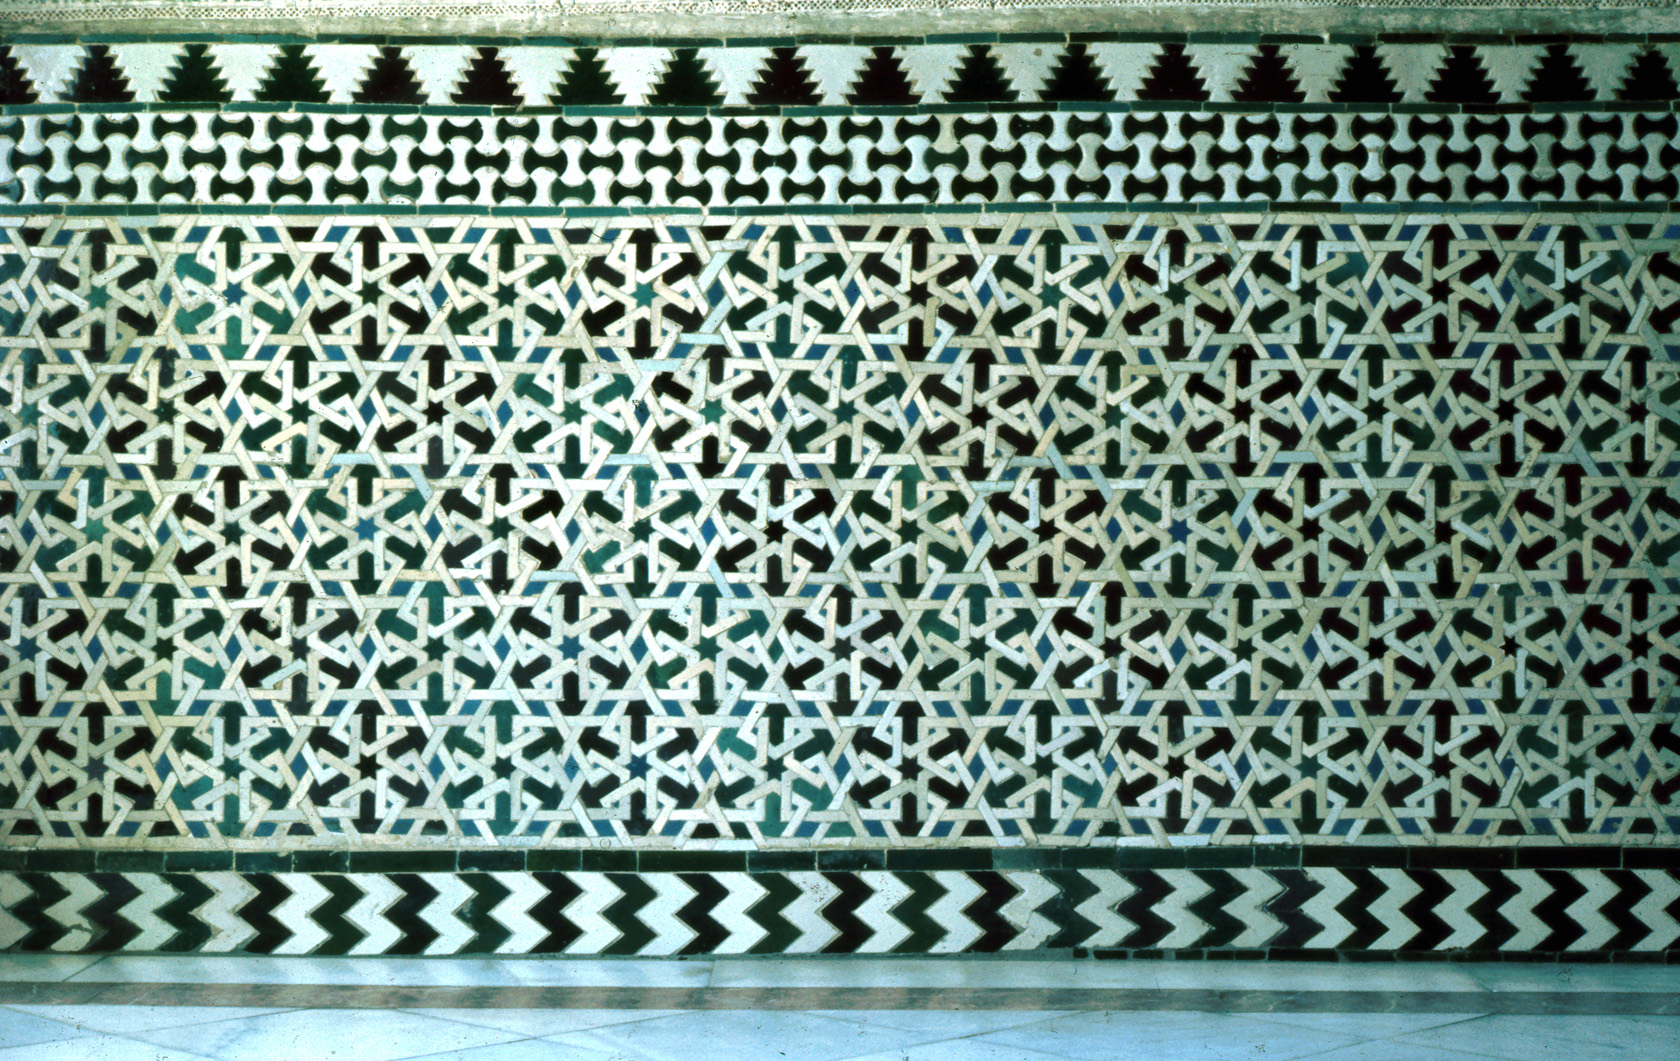
\includegraphics[scale=9]{Alcazar.png}}}
           \only<2>{\put(-125,-80){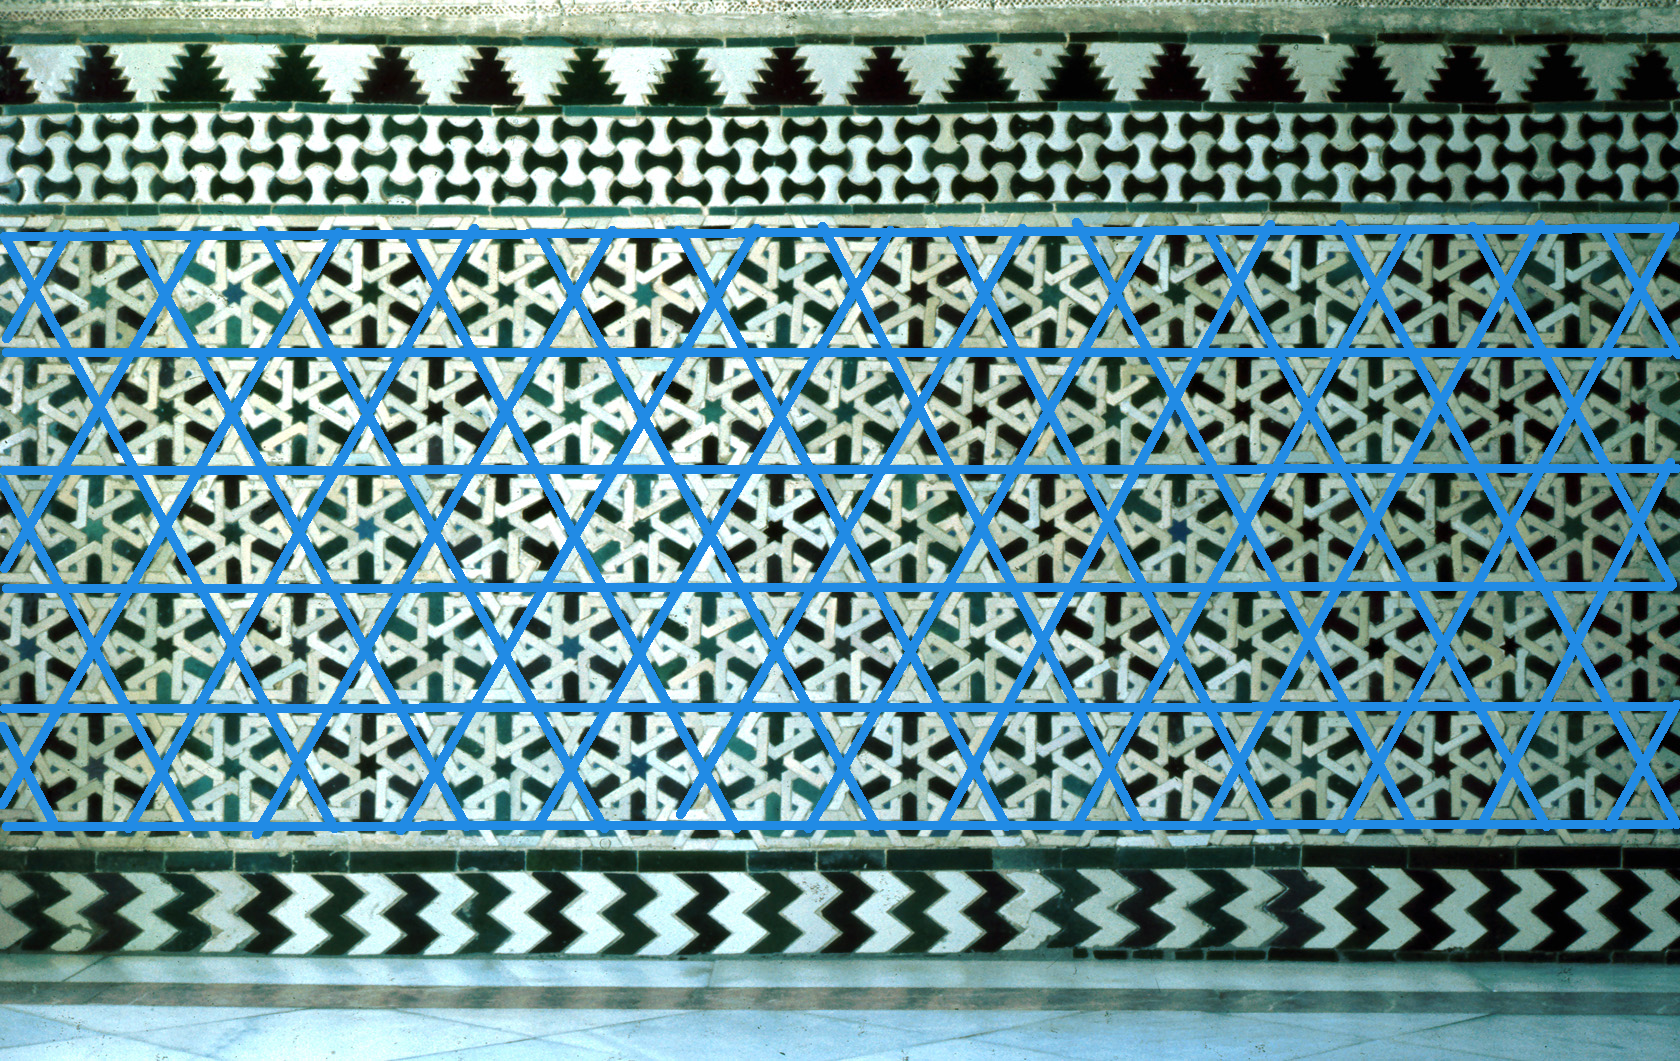
\includegraphics[scale=9]{Alcazar-Kagome.png}}}
           \only<3>{\put(-112,-80){\includegraphics[scale=0.32]{kagome-svg.png}}}
           \only<4>{\put(-112,-80){\includegraphics[scale=0.32]{kagome-spins-svg.png}}}
           \only<5>{\put(-112,-80){\includegraphics[scale=0.32]{kagome-spins-2-svg.png}}}
         \end{picture}
       \end{center}
     \end{frame}




    \begin{frame}\frametitle{Quantum spins}
	\begin{itemize}
		\item Quantum spin: self-adjoint matrices
                  $S_x,S_y,S_z\in M_{N+1}(\C)$ \[[S_x,S_y]=\frac{2i}{N}S_z\qquad
                    [S_y,S_z]=\frac{2i}{N}S_x\qquad [S_z,S_x]=\frac{2i}{N}S_y.\]
                \item Several spins $\rightarrow$ {\color{myorange} tensor product}.
                    \[S_{x,i}=\underbrace{Id\otimes \cdots\otimes Id}_{i-1}\otimes S_x\otimes
                                                                              \underbrace{Id\otimes
                                                                                \cdots
                                                                              \otimes
                                                                              Id}_{d-i}.\]
                                                                          
                                                                        \item<2>
                                                                          Quantum
                                                                          energy
                                                                          (matrix
                                                                          of
                                                                          size
                                                                          $(N+1)^d$):
                                                                          \[
                                                                            \sum_{i\sim j}S_{i,x}S_{j,x}+S_{i,y}S_{j,y}+S_{i,z}S_{j,z}.\]
                    
      
      \end{itemize}
    \end{frame}
    \begin{frame}
      \frametitle{Toeplitz quantization}
      \begin{itemize}
        \item Physics claim: {\color{myorange} quantum-classical
          correspondence} as $N\to +\infty$.
        
      Prediction (Douçot-Simon 1998): lowest-energy eigenvectors concentrate on
      {\color{myorange} some} classical configurations.

    \item<2> Berezin-Toeplitz operators: quantization of the
      symplectic manifold $\mathbb{S}^2$.
    \end{itemize}
  \end{frame}

 %      \begin{frame}
%         \frametitle{Introduction}
%         \setbeamercovered{transparent}
%         {\footnotesize
%         \begin{description}
%         \item<1>[{[Del19]}] Alix Deleporte. “Low-Energy Spectrum of Toeplitz Operators: The Case
% of Wells.” In: Journal of Spectral Theory 9 (2019).
% \item<1-2> [{[Del17++]}] Alix Deleporte. “Low-Energy Spectrum of Toeplitz Operators with a
% Miniwell.” In: arXiv 1610.05902 (2017).
% \item<1>[{[Del18a++]}] Alix Deleporte. “Quantum Selection for Spin Systems.” In: arXiv
% 1808.00718 (2018).
% \item<1>[{[Del18b++]}] Alix Deleporte. “The Bergman Kernel in Constant Curvature.” In:
% arXiv 1812.06648 (2018).
% \item<1-2>[{[Del18c++]}] Alix Deleporte. “Toeplitz Operators with Analytic Symbols.” In: arXiv
% 1812.07202 (2018).
% \item<1>[{[Del19++]}] Alix Deleporte. “WKB Eigenmode Construction for Analytic Toeplitz
%   Operators.” In: arXiv 1901.07215 (2019).
%         \end{description}}
%       \end{frame}

\section{Results}
\begin{frame}
  \frametitle{Characteristic value}
  \begin{itemize}
  \item Let $f$ be smooth and $Z=\{f=0\}$ One can construct a continuous function $\mu$ on $Z$, which only depends on the Hessian of $f$.
  \item $\mu(x)=\inf \Sp(Op^{\text{flat}}(Hess(f)(x)))$,

    where $Op^{\text{flat}}$ is the quantization on flat space which
    fits at $x$ (in the Kähler case: Bargmann quantization).
  \item<2-> {\color{myorange} Quantum selection}: the ground states of $T_N(f)$
    concentrate only on the subset $Z_{\mu}$ of $Z$ where also $\mu$ is minimal.
  \end{itemize}

\end{frame}

\begin{frame}
  \frametitle{Subprincipal localisation}
  \begin{theorem}[(Deleporte 17)]
    Let $M$ be smooth, let $f\in C^{\infty}(M,\R)$ and let $Z_{\mu}$
    be as above. Let $u_N$ be a ground state of $T_N(f)$.

    For all $U\subset M$ at positive distance from $Z_{\mu}$, one has
    \[
      \int_U
      |u_N|^2=O(N^{-\infty}).
    \]
    In progress: $O(\exp(-c\sqrt{N}))$.
  \end{theorem}
\end{frame}

\begin{frame}
  \frametitle{Z is regular and isotropic}
  Classical normal form: up to a symplectic change of variables, near
  a point, the symbol is of the form
  \[
    \langle p,Q_S(q),p\rangle +\langle
    (x,\xi),Q_F(q),(x,\xi)\rangle+O((p,x,\xi)^3,\]
  where $Q_F$ is unitarily equivalent to a matrix of the form
  \[
    \sum \lambda_j (x_j^2+\xi_j^2)
  \]
  (the
  equivalence does not smoothly depend on $q$).

  If $Q_F$ has no resonances, then one can smoothly reduce $Q_F$.
\end{frame}

\begin{frame}
  \frametitle{Quantum normal form}
  The ground state for $Q_F$ is the standard Gaussian, independently
  on $q$, with eigenvalue $\tr Q_F$.
  \vfill

  Born-Oppenheimer approximation: function of the form
  $\exp(-N|x|^2/2)g(q)$. Then the operator acts as
  \[
    -N^{-2}\langle \nabla,Q_S(q)
      \nabla\rangle+N^{-1}(\tr(Q_F(q))+h_1(q))+l.o.\]
  Here $h_1(q)$ comes from the quantization of the symplectic change
  of variables + change of quantization.
\end{frame}

\begin{frame}
  \frametitle{Quantum normal form II}
  What we are left with:
  
  An operator on $T^*Z$, with semiclassical parameter $N^{-\frac 12}$,
  which is {\color{myorange} operator-valued} (takes values into
  functions of $(x,\xi)$). One can always isolate the lowest-energy
  direction (Born-Oppenheimer approximation).
  \vfill
  (Deleporte 17) Complete expansion for the ground state if the
  effective potential $\tr(Q_F)+h_1$ has a non-degenerate minimum.
\end{frame}

\begin{frame}
  \frametitle{Crossings}
  In the physical example before, $Z$ is not smooth.
  \vfill
  (Deleporte 17) Expansions for the lowest-energy eigenvector in the
  case of two manifolds crossing.
  \vfill
  Example: $p_1^2+p_2^2+q_1^2q_2^2$.
\end{frame}

  \begin{frame}
    \frametitle{Thanks}
    \centering 
    {\Large Thanks for your attention!}
  \end{frame}
  

\end{document}
%%% Local Variables:
%%% mode: latex
%%% TeX-master: t
%%% End:
